
\begin{flushleft}

There are two major parts of an L-systems implementation, firstly there is the L-system rewriter, which takes a defined L-system that complies to a partacular grammar, the starting point will be rewritten a number of times using the set of production rules. The rewriting system will give a set of instructions, sometimes called the resultant string. This resultant string is passed to the second system called the interpreter. The interpreter runs through each character or instruction within the resulting string  and interprets its meaning, this acts as a set of instructions that are carried out by turtle graphics to eventually represent a model of a plant on the screen. This chapter will focus on the rewriting system. This includes formaly defining a context-free grammar which the L-system must obide by. Once the grammar has been formalized, a lexical analyser and parser, similar to those used in interpreters and compilers in computing, can be created to represent the context-free L-system grammar, essentially, creating an compiler for a context-free L-system grammar. Using this compiler we can write an L-system, similar to a computer program, the L-system "program" will be passed into the lexical analyser and then through the parser, where each component of the L-system will be identified and parsed into the appropriate computational structures. If the syntax is valid and the parser is successful, the structures created during parsing will be used to rewrite the L-system to a given generation. If the L-system provided does not match the context-free grammar definition, an appropriate error message can be displayed. \\

\vspace{5mm}

For simple D0L-system seen in section \ref{DOL-system example}, creating a rewriter for a simple DOL-system like this is quite simple, each rewritable symbol is only made up of a single character, and because the D0L-system is deterministic we know that there is no randomess when determining the matching rule. This is just a case of storing the starting string, and then iterating through this string one character at a time and when a symbol matches that in a rule, replace that character with the string provided by the rule. This can be implemented relatively simply, however, to implement the parametric 0L-system, where each instruction is a module with potentually multiple parameters and each parameter could be a mathematical expression, the rewriting system will have to better understand what each part of the L-system is specifying based on the grammar and its context in the L-system. The lexical analyser and parser can be used for this purpose in order to classify each part of the L-system and prepare it for rewriting. \\

\vspace{5mm}

\begin{figure}[htbp]
	{\centering
		\setlength{\fboxrule}{1pt}
		\vspace{7px}
		\fbox{
			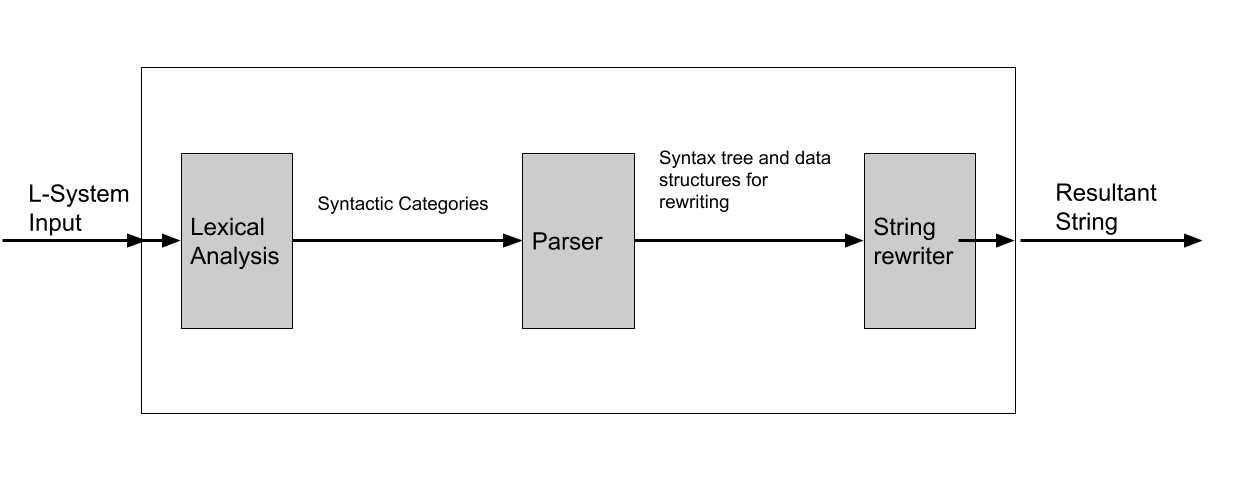
\includegraphics[scale=0.3]{Diagrams/StringRewriter.png}
		}
		\caption{Diagram of the Parts of The Rewiting System.} \label{3D rotations}
	}
\end{figure}
\FloatBarrier

The rewriting system, refers to three specific parts, as seen in the diagram above. The L-system input is passed to the rewriter in the form of a file, or string of text, this string of text is then processed by the lexical analyser, the result of the lexical analyser is a set of syntactic categories which is used by the parser to create the relvent data structures and syntax tree, this information is then used by the string rewriter which finally produces the resultant string that can be interpreted by a domain specific interpreter. Each part of the L-system rewriter will be explained in more detail in following sections. \\

\end{flushleft}

\section{Environment and Tools}

\begin{flushleft}

This majority of the implementation of the L-system will be written in the C and C++ programming languages \cite{stroustrup2000c++}, and I will be using the modern Open Graphics Library or \gls{OpenGL}. The OpenGl framework is one of the industry standards for creating 3D graphics applications, and is a cross platform API for interacting with the \acrshort{gpu} in a low level way. The low level nature of OpenGL is important as some of the structures and models we are going to be displaying and simulating can be graphically intensive \cite{sellers2013opengl} \cite{movania2017opengl}. OpenGL was originally intended to be an \acrshort{api} for the C and C++ programming languages, and therefore we can have a programming language and graphics API which have a strong emphasis on performance.

\vspace{5mm}

There are also a number of libraries which will provide some extra functionality. The standard library for C and C++ provides many usefull structures and functions which will be incredibly usefull during the development process. For more specialised mathematics capabilities the \acrfull{glm} library holds many mathematics classes and functions for conveniently dealing with some 3D mathematics such as vectors, matrices and quaternions. Another important library is the \acrfull{glfw} which is a multiplatform \acrshort{api} for creating an managing user interface windows, events and user input \cite{glfwDocumentation}.

\vspace{5mm}

In order to keep track of changes and manage versions Git is a free and open source version control software, that is able to keep track of changes that have been made to the files within a project folder. It will be used to keep track of previous versions of the project throughout the development process. Git can be used in conjuction with Github, which is a online web application that stores git repositories. This acts as a backup as well as containing all previous versions of the project \cite{torvalds}.

\end{flushleft}

\section{The L-system as an interpreted grammar}

\begin{flushleft}

Traditionally an interpreter in computing is a program that takes program code as input, where it is then analyzed and interpreted as it is encountered in the execution process. All of the previously encountered information is kept for later interpretations. The information about the program can be extracted by inspection of the program as a whole, such as the set of declared variables in a block, a function, etc \cite{wilhelm2010compiler}. In essence, the L-system rewriter contains a type of interpreter, this should not be confused with the interpreter that processes the resultant string using turtle graphics. Due to this confusion of terms I will refer the system containing the lexical analyser, L-system parser and the string rewriter as the L-system rewriter, instead of an interpreter in the computational sense. \\

\vspace{5mm}

A similarity can be drawn between traditional interpreted languages and the L-system rewriter. The L-system rewriter defines a set of constant variables, a starting point and then some production rules. This information can then be used to rewrite the starting string a number of times. Later on, it may be decided that, instead of five generations of rewriting, the rewriter should instead generate ten rewrites. Some information about the L-system is still valid, the production rules, axiom and constants have not changed and therefore, this information can be used in order to interpret to the tenth generation instead. This can be used to go from the current state of the L-system rewriter and just rewrite another five times. Instead of throwing all the information away and starting from scratch. Furthermore, if we would like to retrieve the resultant string, this can simply be asked for from the L-system rewriter. \\

\vspace{5mm}

The lexical analyser and parser are a neccessary part in order to carry out rewriting. Without them it would be difficult to find the syntactic roles of each part of the L-system, take the module: F(2*3, x * (2 + y)) as an example, here there is a single module with two parameters, one parameter has the expression (2 * 3) and the other has the expression (x * (2+y)), these complex structures within a grammar require knowledge about the structure of the grammar it represents. The lexical analyser firstly makes sure that all the syntax within the L-system is correct and assigns each word or symbol to a syntactic category, the parser then splits the L-system into its component parts and is describes each parts syntactic roll. This provides the understanding that x and y are variables within a module and do not represent another module, as well as where the values of x and y could be found. \\

\vspace{5mm}

The trade off of creating an L-system with more complexity within the grammar itself is that it become more difficult to write a valid L-system to represent a particular structure, the advantage of using an rewriter specifically designed for a \acrshort{cfg} like the parametric 0L-system grammar is that it can make it simpler to debug any syntactic errors within an L-system, as well as make the string rewriting much faster. This means that writing a L-system becomes simlar to rewriting a recursive program and any syntactic mistakes made in writing this \say{program} results in a meaningful error describing what was incorrect. \\

\end{flushleft}

\section{The Syntax of a Parametric L-system}

\begin{flushleft}

This section will cover the valid syntax for the parametric L-system rewriter, the syntax for the parametric 0L-system is similar to the definition of the L-systems given by Prusinkiewicz and Lindenmayer in section \ref{definition of a parametric 0L-system section}, this is to keep consistant with how most L-systems are defined. There are some additions and modifications to the syntax definition provided by Prusinkiewicz and Lindenmayer in order to construct a L-system that includes branching, constant variable definitions, object specifications, parametric L-system concepts, randomness as well as stochastic L-systems \cite{prusinkiewicz2012algorithmic}. \\

\vspace{5mm}

This parametric 0L-system is made up of five major parts, each part can be catagorised as a statement, these statements are the define statements, include statements, a single generation statement, a single axiom statement and a one or more production rule statements \cite{prusinkiewicz2013lindenmayer}. All of these statements collectively form a parametric 0L-system. Each statement starts with a \# character and ends with a ; character, this is useful to the lexer and parser and allows two statements to be written on the same line. \\ 

\vspace{5mm}

The order of statements should be listed as follows: \\

\vspace{5mm}

\begin{equation} \label{statement order example}
\begin{aligned}
	&\text{\#generations statement;}\\
	&\text{\#define statements;}\\
	&\text{\hspace{10mm}...}\\
	&\text{\#include statements;}\\
	&\text{\hspace{10mm}...}\\
	&\text{\#axiom statement;}\\
	&\text{\#production statements;}\\
	&\text{\hspace{10mm}...}\\
\end{aligned}
\end{equation}

\vspace{5mm}

The order for some of statments does not necessarily matter, such as the generations statement which can be defined anywhere within the L-system, however, there are some parts that are required to be in a particular order, for instance, the define and include statements must appear above the axiom and productions statements as they define values used within the axiom and production rules. It is best practice to specify the L-system in the above order as to avoid any conflictions or errors. \\

\vspace{5mm}

Another design decision that has been made, is that all numbers within the L-system are repersented as floating point numbers. Other data types could be added to the definition of the L-system in the future, however, there is some added complexities in doing so, such as the conversion from one type to another, or having to specify which data type a variable represents. For all intents and purposes, the floating point data type provides all the neccessary functionality needed for the L-system, therefore, it seems unnecessary to add extra data types. \\

\end{flushleft}

\section{Scanner - Flex} \label{Flex}

\begin{flushleft}

D. Cooper and L. Torczon write that "The scanner, or lexical analyser, reads a stream of characters and produces a streeam of words. It aggregates characters to form words and applies a set of rules to determin wheter or not each word is legal in the source language. If the word is valid, the scanner assigns it a syntactic category, or part of speech" \cite{cooper2011engineering}. The lexer for parametric 0L-system will need to do exactly that. To get to a stage where we can successfully rewrite the L-system string, the rewriter must first understand what each word and symbol represents, in the form of a syntactic category, and whether or not the word or symbol is valid or not. \\

\vspace{5mm}

It is possible to write custom \gls{Lexer}, however, it can be quite complicated and time consuming to design and implement, and once a custom \gls{Lexer} has been created it can be difficult to change functionality at a later stage. Luckely there is a well known program known as the \acrlong{flex} (\acrshort{flex}), \acrshort{flex} takes in a file which contains the lexical rules of the language, it uses these rules to create a \gls{Lexer} program. When \acrshort{flex} is run it will create a \gls{Lexer} in the form of a C program. We can use the generated Lexer on the L-system that we would like to rewrite, taking the word within the L-system and assigning a syntactic category to it. In order to create a lexer with \acrshort{flex}, the lexical rules in the form of syntactic categories must defined. Below are the valid syntactic categories of a parametric 0L-system:

\begin{table}[h!] \center
\begin{tabular}{ | c | l | l |}
\hline
	Syntactic Word	& Syntactic Category & Meaning\\  
\hline
\hline
	, 				& T\_COMMA 				& Separation between module parameters \\
\hline
	: 				& T\_COLON 				& Separation between production rule parts \\
\hline
	; 				& T\_SEMI\_COLON 		& End of a statement\\
\hline
	\#				& T\_HASH 				& Beginning of a statement\\
\hline
	( 				& T\_PARENL 			& Start of a modules parameters \\
					&						& or specifies presidence in an expression \\
\hline
	) 				& T\_PARENR 			& End of a modules parameters \\
					&						& or specifies presidence in an expression \\
\hline 
	\{ 				& T\_BRACKETL 			& Start of a random range\\
\hline
	\} 				& T\_BRACKETR 			& End of a random range\\
\hline
	$\sim$ 			& T\_TILDE 				& Stochastic operator\\
\hline
	== 				& T\_EQUAL\_TO 			& Relational operator stating equal to\\
\hline
	!= 				& T\_NOT\_EQUAL\_TO 	& Relational operator for not equal to\\
\hline		
	$<$ 			& T\_LESS\_THAN 		& Relational operator for less than\\
\hline
	$>$ 			& T\_GREATER\_THAN 		& Relational operator for greater than\\
\hline
	$<$ = 			& T\_LESS\_EQUAL 		& Relational operator for greater or equal\\
\hline
	$>$ = 			& T\_GREATER\_EQUAL 	& Relational operator for greater or equal\\
\hline
	[ 				& T\_SQUARE\_BRACEL 	& Module name (branching save state) \\
\hline
	] 				& T\_SQUARE\_BRACER 	& Module name (branching load state) \\
\hline
	+ 				& T\_PLUS 				& Arithmetic operator for addition, or\\
					&						& Module name (Yaw right) \\
\hline
	- 				& T\_MINUS 				& Arithmetic operator for subtraction, or\\
					&						& Module name (Yaw left)\\
\hline
	/ 				& T\_FORWARD\_SLASH 	& Arithmetic operator for division, or\\
					&						& Module name (Pitch up)\\
\hline
	$\backslash$ 		& T\_BACK\_SLASH 		& Module name (Pitch down)\\
\hline
	* 				& T\_STAR 				& Arithmetic operator for multiplication, or\\
					&						& Condition in a production rule which is true\\
\hline
	$\land$ 		& T\_HAT 				& Arithmetic operator for and exponent, or\\
					&						& Module name (Roll right)\\
\hline
	$\&$ 			& T\_AMPERSAND 			& Module name (Roll left)\\
\hline
	! 				& T\_EXCLAMATION 		& Module name (Set size of branch)\\
\hline
	\$ 				& T\_DOLLAR 			& Module name \\
\hline
	= 				& T\_ASSIGN 			& Assignment operator used to set generations\\
\hline
	\#n 			& T\_GENERATIONS 		& Declaration of the number of generations\\
\hline
	\#w 			& T\_AXIOM 				& Declaration of the axiom\\
\hline
	\#define 			& T\_DEFINE 		& Declaration of the define\\
\hline
	\#object 			& T\_OBJECT			& Declaration of the object\\
\hline
	[0-9]+\.[0-9]+|[0-9]+ 					& T\_FLOAT 				& Regular expression for a floating point number\\
\hline
	[a-zA-Z\_][a-zA-Z0-9\_]*  				& T\_VAR\_NAME 			& Regular expression for a module or variable name\\
\hline
\hline
\end{tabular}
\caption{Table of Valid Lexer Words}
\label{lexer words}
\end{table}
\FloatBarrier

From the table above there are a number syntactic categories which contain more than one meaning to the grammar, for instance the ( and ) parenthesis have two meanings, it is either to specify the begining and end of a modules parameters or it specifies presidence within an expression.  It is not up to the scanner to determine what the each particular parentheses means, or that it has a meaning at all, the lexer only recognises that it falls into the syntactic categories, T\_PARENL and T\_PARENR. Deriving the meaning of a given token or sytactic category is left up to the parser which is more aware of the context of each syntactic word. Similarly, the symbols [,],+,-,/,$\backslash$, $\land$, $\&$, ! and \$ are valid module names; Moreover, it is possible for a T\_VAR\_NAME to also be a module name, these symbols need to be specifically defined as their own syntactic category, as they not only represent a module name but can also represent a different meaning depending on their context. For instance, the +, -, / are valid module names, but they also are mathematical symbols used within an arithmetic expression. The scanner must separate these symbols and keep them in their own syntactic category in order for the parser to be able to understand the same symbol in multiple contexts. \\

\vspace{5mm}


It is also important to note that there are two special types of tokens, these being the T\_FLOAT and T\_VAR\_NAME which not only are part of a syntactic category but also contain a value, for instance T\_FLOAT has a floating point value and T\_VAR\_NAME has a string value. These values must be kept and provided to the parser.\\

\end{flushleft}

\section{Parser - Bison} \label{Bison}

The parsers job is to find out if the input stream of words from the \gls{Lexer} makes up a valid sentence in the language. The \gls{Parser} fits the syntactical category to the grammatical model of the language. If the \gls{Parser} is able to fit the syntactical category of the word to the grammatical model of the language then the syntax is seen to be correct. If all of the syntax is correct the \gls{Parser} will output a syntax tree and build the structures for use later on during the compilation process \cite{cooper2011engineering}.

\subsection{Building a Generalised L-system Grammar}

We are now able to represent complex three dimensional tree structures in the form of a L-system rule set. In a computing sense this rule set can be seen as a type of program. In the program we define the number of generations we would like to generate, the starting point (Axiom) some constant varables (\#define) and the set of production rules. \\
Using this information, we iterate through the from generation to generation rewritting the strings and then at the end provide a resulting string which will then be interpreted and displayed on the screen.
\\
We can represent the languages grammar in the form of a \acrlong{bnf}, \acrshort{bnf} is a notation for \acrlong{cfg}s used to describe the syntax of different languages. In this case the \acrshort{bnf} is used below to describe the syntax of the parametric L-system grammar. \\
\\
For example: \\ 
\\
\textless expression\textgreater~ $\rightarrow$ number \\ 
\textless expression\textgreater~ $\rightarrow$ (\textless expression\textgreater~) \\
\textless expression\textgreater~ $\rightarrow$ \textless expression\textgreater~ + \textless expression\textgreater~ \\
\textless expression\textgreater~ $\rightarrow$ \textless expression\textgreater~ - \textless expression\textgreater~ \\
\\
The first line states that an \textless expression\textgreater~ can be any number, line two states that an \\ \textless expression\textgreater~ can also be an expression that is inside parenthesis. Line three states that an \\ \textless expression\textgreater~ can be an \textless expression\textgreater~ added to another \textless expression\textgreater~, furthermore line four states that an \textless expression\textgreater~ can also be an \textless expression\textgreater~ subtracted by another \textless expression\textgreater~. \\
\\
The above grammar can be expressed as follows: \\
\\
\textless expression\textgreater~ $\rightarrow$ number 

\hspace{2cm} $|$ (\textless expression\textgreater~) 

\hspace{2cm} $|$ \textless expression\textgreater~ + \textless expression\textgreater~ 

\hspace{2cm} $|$ \textless expression\textgreater~ - \textless expression\textgreater~ \\
\\
Here the $|$ symbol can be articulated as an OR, therefore it can be said that an \textless expression\textgreater~ can be a number OR an \textless expression\textgreater~ surrounded by parenthesis, OR an \textless expression\textgreater~ added to another \textless expression\textgreater~ OR an \textless expression\textgreater~ subtracted by another \textless expression\textgreater~. 
\\
In addition to this, any statement that is not surrounded by \textless \textgreater, states it must match that particular string. The $\in$ followed by an $|$ states that it can either be nothing or another statement. \\
\\

\subsection{\acrlong{bnf} of the L-system Grammar} \label{L-system Grammar}

	$<$prog$>$ $\rightarrow~ \in$ \\
	\hspace{2cm} $|$ $<$statements$>$ EOF \\
	
	\noindent
	$<$statements$>$ $\rightarrow~$ $\in$ \\
	\hspace{2cm} $|$ $<$statement$>$ $<$statements$>$ \\ 
	
	\noindent
	$<$statement$>$ $\rightarrow$~ EOL \\
	\hspace{2cm} $|$ $<$generations$>$ \\ 
	\hspace{2cm} $|$ $<$definition$>$ \\ 
	\hspace{2cm} $|$ $<$object$>$ \\ 
	\hspace{2cm} $|$ $<$axiom$>$ \\ 
	\hspace{2cm} $|$ $<$production$>$ \\ 
	
	\noindent
	$<$generations$>$ $\rightarrow$ T\_GENERATIONS T\_ASSIGN T\_FLOAT T\_SEMI\_COLON \\
	\noindent
	$<$number$>$ $\rightarrow$ T\_FLOAT \\
	\hspace{2cm} $|$ T\_MINUS T\_FLOAT \\ 
	
	\noindent
	$<$range$>$ $\rightarrow$ T\_BRACEL $<$number$>$ T\_COMMA $<$number$>$ T\_BRACER\\
	
	\noindent
	$<$definition$>$ $\rightarrow$ T\_DEFINE T\_VAR\_NAME $<$number$>$ T\_SEMI\_COLON \\
	\hspace{2cm} $|$  T\_DEFINE T\_VAR\_NAME $<$range$>$ T\_SEMI\_COLON \\
	
	\noindent
	$<$object$>$ $\rightarrow$ T\_OBJECT T\_VAR\_NAME T\_VAR\_NAME T\_SEMI\_COLON \\
	
	\noindent
	$<$module$>$ T\_VAR\_NAME \\
	\hspace{2cm} $|$ T\_PLUS \\ 
	\hspace{2cm} $|$ T\_MINUS \\ 
	\hspace{2cm} $|$ T\_FORWARD\_SLASH\\ 
	\hspace{2cm} $|$ T\_BACK\_SLASH \\ 
	\hspace{2cm} $|$ T\_HAT \\ 
	\hspace{2cm} $|$ T\_AMPERSAND \\ 
	\hspace{2cm} $|$ T\_DOLLAR \\ 
	\hspace{2cm} $|$ T\_SQUARE\_BRACEL \\ 
	\hspace{2cm} $|$ T\_SQUARE\_BRACER \\ 
	\hspace{2cm} $|$ T\_EXCLAMATION \\ 
	\hspace{2cm} $|$ T\_VAR\_NAME T\_PARENL $<$param$>$ $<$param\_list$>$ T\_PARENR\\ 
	\hspace{2cm} $|$ T\_PLUS $<$param$>$ $<$param\_list$>$ T\_PARENR\\ 
	\hspace{2cm} $|$ T\_MINUS $<$param$>$ $<$param\_list$>$ T\_PARENR\\ 
	\hspace{2cm} $|$ T\_FORWARD\_SLASH $<$param$>$ $<$param\_list$>$ T\_PARENR\\ 
	\hspace{2cm} $|$ T\_BACK\_SLASH $<$param$>$ $<$param\_list$>$ T\_PARENR\\ 
	\hspace{2cm} $|$ T\_HAT $<$param$>$ $<$param\_list$>$ T\_PARENR\\ 
	\hspace{2cm} $|$ T\_AMPERSAND $<$param$>$ $<$param\_list$>$ T\_PARENR\\ 
	\hspace{2cm} $|$ T\_DOLLAR $<$param$>$ $<$param\_list$>$ T\_PARENR\\ 
	\hspace{2cm} $|$ T\_SQUARE\_BRACEL $<$param$>$ $<$param\_list$>$ T\_PARENR\\ 
	\hspace{2cm} $|$ T\_SQUARE\_BRACER $<$param$>$ $<$param\_list$>$ T\_PARENR\\ 
	\hspace{2cm} $|$ T\_EXCLAMATION $<$param$>$ $<$param\_list$>$ T\_PARENR\\ 



% Axiom
\noindent
\textless axiom\textgreater~ $\rightarrow$  \#w : \textless axiom statement list\textgreater~ ; \\



% Axiom Statement List
\noindent
\textless axiom statement list\textgreater~ $\rightarrow$ $\in$ 

\hspace{2cm} $|$ \textless axiom statement\textgreater~ \textless axiom statement list\textgreater~ ; \\



% Axiom Statement
\noindent
\textless axiom statement\textgreater~ $\rightarrow$ \textless moduleAx\textgreater~ \\



% Axiom Module 
\noindent
\textless moduleAx\textgreater~  $\rightarrow$ \textless variable\textgreater~ $|$ "$+$" $|$ "$-$" $|$ "/" $|$ "$\backslash$" $|$ "\textasciicircum" $|$ "$\&$" $|$ "!" 

\hspace{2cm} $|$ \textless variable\textgreater~ (  \textless paramAx\textgreater~ \textless paramListAx\textgreater~ )

\hspace{2cm} $|$ +(  \textless paramAx\textgreater~ \textless paramListAx\textgreater~ ) 

\hspace{2cm} $|$ -(  \textless paramAx\textgreater~ \textless paramListAx\textgreater~ ) 

\hspace{2cm} $|$ /(  \textless paramAx\textgreater~ \textless paramListAx\textgreater~ ) 

\hspace{2cm} $|$ $\backslash$(  \textless paramAx\textgreater~ \textless paramListAx\textgreater~ )

\hspace{2cm} $|$ \textasciicircum (  \textless paramAx\textgreater~ \textless paramListAx\textgreater~ ) 

\hspace{2cm} $|$ $\&$(  \textless paramAx\textgreater~ \textless paramListAx\textgreater~ ) \\



% Axiom Parameter List
\noindent
\textless paramAxList\textgreater~ $\rightarrow$  $\in$ 

\hspace{2cm} $|$ , \textless paramAx\textgreater~ \textless paramAxList\textgreater~ \\



% Axiom Parameter
\noindent
\textless paramAx\textgreater~ $\rightarrow$ \textless expression\textgreater~ \\



% Production
\noindent
\textless production\textgreater~ $\rightarrow$  \# \textless variable\textgreater~  : \textless predecessor\textgreater~ : \textless condition\textgreater~  : \textless successor\textgreater~ ;\\



% Predecessor
\noindent
\textless predecessor\textgreater~ $\rightarrow$ \textless pred statement list\textgreater~ \\


% Predecessor Statement List
\noindent
\textless pred statement list\textgreater~ $\rightarrow$ $\in$

\hspace{2cm} $|$ \textless pred statement\textgreater~ \textless pred statement list\textgreater~ \\


% Predecessor Statement
\noindent
\textless pred statement\textgreater~ $\rightarrow$ \textless module\textgreater~ \\



% Condition 
\noindent
\textless condition\textgreater~ $\rightarrow$ *

\hspace{2cm} $|$ \textless left expression\textgreater~ \textless conditions statement\textgreater~ \textless right expression\textgreater~ \\


% Condition Left Expression
\noindent
\textless left expression\textgreater~ $\rightarrow$ \textless expression\textgreater~ \\


% Condition Right Expression
\noindent
\textless right expression\textgreater~ $\rightarrow$ \textless expression\textgreater~ \\


% Condition Statement
\noindent
\textless condition statement\textgreater~ $\rightarrow$ == $|$ != $|$ \textless $|$ \textgreater $|$ \textless = $|$ \textgreater =\\



% Successor
\noindent
\textless successor \textgreater~ $\rightarrow$ \textless successor statement list \textgreater~ \\


% Successor Statement List
\noindent
\textless successor statement list\textgreater~ $\rightarrow$ $\in$

\hspace{2cm} $|$ \textless successor statement\textgreater~ \textless successor statement list \textgreater~ \\


%Successor Statement
\noindent
\textless successor statement\textgreater~ $\rightarrow$ \textless module\textgreater~ \\



% Module
\noindent
\textless module\textgreater~ $\rightarrow$  \textless variable\textgreater~ $|$ $+$ $|$ $-$ $|$ / $|$ $\backslash$ $|$ \textasciicircum $|$ $\&$ $|$ ! 

\hspace{2cm} $|$ \textless variable\textgreater~ (  \textless param\textgreater~ \textless paramList\textgreater~ )

\hspace{2cm} $|$ +(  \textless param\textgreater~ \textless paramList\textgreater~ )

\hspace{2cm} $|$ -(  \textless param\textgreater~ \textless paramList\textgreater~ )

\hspace{2cm} $|$ /(  \textless param\textgreater~ \textless paramList\textgreater~ ) 

\hspace{2cm} $|$ $\backslash$(  \textless param\textgreater~ \textless paramList\textgreater~ ) 

\hspace{2cm} $|$ \textasciicircum (  \textless param\textgreater~ \textless paramList\textgreater~ ) 

\hspace{2cm} $|$ $\&$(  \textless param\textgreater~ \textless paramList\textgreater~ ) \\



% Parameter List
\noindent
\textless paramList\textgreater~ $\rightarrow$ $\in$ $|$ : \textless param\textgreater~ \textless paramList\textgreater~ \\



%Parameter List
\noindent
\textless param\textgreater~ $\rightarrow$ \textless expression\textgreater~ \\



% Expression
\noindent
\textless expression\textgreater~ $\rightarrow$  \textless variable\textgreater~

\hspace{2cm} $|$ \textless float\textgreater~

\hspace{2cm} $|$ \textless expression\textgreater~ + \textless expression\textgreater~

\hspace{2cm} $|$ \textless expression\textgreater~ - \textless expression\textgreater~

\hspace{2cm} $|$ \textless expression\textgreater~ * \textless expression\textgreater~

\hspace{2cm} $|$ \textless expression\textgreater~ / \textless expression\textgreater~

\hspace{2cm} $|$ \textless expression\textgreater~ \textasciicircum \textless expression\textgreater~

\hspace{2cm} $|$ "(" \textless expression\textgreater~ ) \\



% Float
\noindent
\textless float\textgreater~ $\rightarrow$ [0-9]+.[0-9]+ \\



% Variable
\noindent
\textless variable\textgreater~ $\rightarrow$ [a-zA-Z\_][a-zA-Z0-9\_]* \\

\subsection{Constants and Objects}

\begin{flushleft}

Defining constants and objects is similar syntactically, the keyword define or include is used, followed by a variable name followed by a value, the value for a constant is a floating point number and the value for an include is a name of an object within the predefined object library. An example of the defining a constant and an object can be seen below: \\

\begin{equation} \label{constant and object example}
\begin{aligned}
	&\text{\#define num 10;}\\
	&\text{\#define pi 3.1415;}\\
	&\\
	&\text{\#include F BRANCH;}\\
	&\text{\#include S SPHERE;}\\
\end{aligned}
\end{equation}

The definition variables can be stored as a table, called a constants table, which keeps track of all of the constant variable names as well as their values defined by the L-system, as seen in the table below: \\

\vspace{5mm}

\begin{table}[h!] \center
\begin{tabular}{ | c | l | }
\hline
	Variable Name 	& Value\\  
\hline
\hline
	num 				& 10.0\\
\hline
	pi					& 3.1415\\
\hline
\end{tabular}
\caption{Table of turtle instruction symbols and their meaning to the interpreter}
\label{constants table}
\end{table}
\FloatBarrier

The object table structure is very similar to the constants table, the object table holds the module name, and name of the object in the predefined object library. The object table will not be used during rewriting but will be necessary to provide information during the interpretation of the resulting string about which objects each module should render. \\

\begin{table}[h!] \center
\begin{tabular}{ | c | l | }
\hline
	Module Name	& Object Name\\  
\hline
\hline
	F 				& BRANCH\\
\hline
	S				& SPHERE\\
\hline
\end{tabular}
\caption{Table of turtle instruction symbols and their meaning to the interpreter}
\label{constants table}
\end{table}
\FloatBarrier

\end{flushleft}

\subsection{Modules and Strings}

\begin{flushleft}

For the purposes of the rewriter it is important to understand that there are three major parts of a module, there is a module name, which is a string of characters or a symbol, secondly there is a list of parameters signified by open and close parenthesis, there can be zero or more parameters listed. If there are no parameters for a module you can specify it without parenthesis, however, there should then be a space between the module without parenthesis and the next module. Thirdly, each parameter can either be made up of a number, variable, random number range or a mathematical expression containing  numbers, variables and parentheses signifying precedence. \\   

\vspace{5mm}

There are two types of modules, one being a module definition and the other a module call. The module definition stands as a type of template of a module within a production rule, these templates do not have to hold actual values but the values will be substituted during the rewriting process. The module calls would appear either in the axiom or in the resultant string, the parameters of a module call will hold an actual numerical value. Below is an example outlining the difference between the module definition and module calls.\\ 

\begin{equation} \label{module definition and call example}
\begin{aligned}
	&\text{\#w : A(10);}\\
	&\text{\#p1 : A(x) : * : A(x)A(x); }\\
\end{aligned}
\end{equation}

In example \ref{module definition and call example} above, the module A(10) within the axiom, is a module call, as it contains the numerical value of 10 in the first parameter. In the production rule p1 the module A(x) within the predecessor is a module definition, it states that module A's first parmeter has a local variable x, the calling modules value will substitute x and will replace the value of x anywhere within the successor statement, p1's successor has two modules A(x)A(x), also module defintions however the value x will be subtituted with the calling modules value. When a production rules successor rewrites the calling module, the successors modules must have a numerical value, they then become module calls within the resultant string. \\ 

\vspace{5mm}

A string in the context of a parametric L-system is a vector of modules, this being the C++ standard library vector data structure. The modules are linked one after the other creating a type of string, but instead of characters or symbols we have a string of modules. \\

\end{flushleft}